% Anonymized manuscript for the Journal of Information Science (SAGE). Identifying details are in title_page.tex.
% Build: tectonic saga_manuscript.tex   or   latexmk -pdf saga_manuscript.tex   (or upload this folder to Overleaf)
% Numbers in tables/ and figures/ are generated: scripts/eval_all.py -> significance.py -> make_tables.py / make_figures.py
\documentclass[Afour,sagev,times]{sagej}

% sagej.cls already loads natbib (numbers, sorted and compressed) for the sagev option
% T1 makes the class's Times fonts available under XeTeX-based engines (tectonic) as well as pdfLaTeX
\usepackage[T1]{fontenc}
\usepackage{url}

\usepackage[colorlinks,bookmarksopen,bookmarksnumbered,citecolor=red,urlcolor=red]{hyperref}


\begin{document}
\title{Typed Decision Models as Passage Rerankers: Effectiveness, Calibration, and Context Selection}

\author{Anonymous submission}


\begin{abstract}
Typed decision models return probabilities over caller-defined options.
We test four families as pointwise rerankers of BM25 top-100 candidates from 13 TREC DL and BEIR collections.
Jev averages 55.3--56.1 nDCG@10, on par with Qwen3-Reranker-8B (56.0) and above bge-reranker-v2-m3 (53.7), varying widely by collection.
Clef does not differ significantly from its base on six of seven collections; Jeff improves on its base.
Jev's raw yes/no probabilities have lower calibration error than bge's (15.0 vs.\ 20.0), but bge calibrated on same-threshold collections closes this gap, and prompt rewording moves it by more.
In retrieval-augmented generation on a family-disjoint MuSiQue split, Jev raises multi-hop F1 over bge in all 27 policy--generator pairs (23 significant with family-clustered Holm tests) and over Qwen3-Reranker-8B in 26 (12 significant); on NQ, one of 27 is significant.
Probability thresholds do not beat fixed top-$k$.
Typed decision models are competitive rerankers, but calibration alone does not improve context selection.

\end{abstract}

\keywords{reranking, decision models, calibration, retrieval-augmented generation, BEIR}

\maketitle

\section{Introduction}

Retrieval-augmented generation (RAG) pipelines typically retrieve candidates with a cheap first stage, rerank them with a cross-encoder\cite{nogueira2019monobert} or an LLM\cite{sun2023rankgpt}, and pass a fixed top-$k$ to the generator.
Two weaknesses of this recipe are well known: cross-encoders trained on MS~MARCO transfer imperfectly to new domains\cite{thakur2021beir}, and their scores are not probabilities\cite{penha2021calibration}, so the cut-off $k$ is chosen by habit rather than by evidence.

A recently released class of models targets both: \emph{typed decision models} such as Jev\cite{jev}, Cloudflare Clef\cite{clef}, Jeff\cite{jeff}, and Laya\cite{laya}.
Instead of generating text, they answer a typed question about a state---a choice among named options, a yes/no (Noul) question, or an ordered scale---and return per-option probabilities.
A relevance judgment is a natural typed question (\emph{Is this passage relevant to the query?}), and a per-option probability is exactly what a context-selection rule such as ``keep passages with $P(\text{relevant})>t$'' needs. Whether that probability is actually calibrated, and whether such a threshold beats a fixed cut-off, are empirical questions that the interface alone does not answer.

Evidence so far is thin: decision models have been evaluated for recommendation reranking\cite{lyu2026jevrec} and agent-memory selection\cite{sharma2026selection}, a practitioner blog reports Jev results on two BEIR datasets\cite{denser2026jevqwen}, and an early audit finds that typed readouts have not yet shown an accuracy advantage over comparable label-probability readouts\cite{tang2026tdmaudit}.
No systematic study has evaluated decision models as passage rerankers on standard IR benchmarks against cross-encoders and label-probability LLM rerankers, or measured whether their relevance probabilities are calibrated.

We provide that study, organized around three research questions.
\textbf{RQ1:} Can typed decision models, used without task-specific tuning as pointwise rerankers, match cross-encoders and label-probability LLM rerankers?
\textbf{RQ2:} Are their relevance probabilities calibrated, with and without labels from the target collection?
\textbf{RQ3:} Do these probabilities help decide which passages a retrieval-augmented generator should see?
Our contributions and main findings are:
(1)~An evaluation of four decision-model families and three question formats on 13 collections against cross-encoders and label-probability LLM rerankers, with same-base controls for Clef and Jeff and equal-context ablations. The large decision models are on par on average with the strongest label-probability reranker we run on all 13 collections, a 4-bit Qwen3-Reranker-8B, with large differences on individual collections; Clef is close to its own base LLM, and Jev's base is unknown.
(2)~A calibration analysis on nine collections with judged negatives. Raw yes/no probabilities from Jev and Laya are better calibrated than raw cross-encoder scores, but a cross-encoder calibrated on other collections with the same relevance threshold closes the gap, so the practical advantage is not needing labelled source data; raw calibration also depends strongly on the prompt wording.
(3)~A RAG evaluation on MuSiQue and NQ with three generators, comparing fixed top-$k$, gap-based, and threshold-based context selection. Jev's rankings help multi-hop QA more than those of bge-reranker-v2-m3 or the equally effective Qwen3-Reranker-8B, including on a family-disjoint split, and Jev more often ranks the answer-bearing hop first, yet probability thresholds do not beat fixed $k$.
(4)~Code for reproducing and extending the evaluation, with input hashes, split IDs, and all statistical outputs.

\section{Related Work}

\paragraph{Neural and LLM reranking.}
Cross-encoders score each query--passage pair jointly~\cite{nogueira2019monobert,nogueira2020monot5} and remain the default second stage; BEIR showed that their in-domain gains shrink out of domain~\cite{thakur2021beir}.
LLM rerankers can be pointwise, pairwise, setwise, or listwise: RankGPT's sliding-window listwise prompting is competitive with supervised rerankers~\cite{sun2023rankgpt}, distilled listwise models such as RankZephyr and FIRST make this cheaper~\cite{pradeep2023rankzephyr,reddy2024first}, and setwise prompting trades off the two~\cite{zhuang2023setwise}.
Pointwise LLM rankers read relevance from the probability of a ``yes'' token and improve with graded rather than binary labels~\cite{zhuang2023beyond}; Qwen3-Reranker is a recent model trained for exactly this readout~\cite{qwen3embedding}.
Typed decision models are also pointwise, but their answer space is a declared set of options, each of which receives a probability by construction; we compare them directly with label-probability rerankers.

\paragraph{LLMs as relevance assessors.}
LLMs can predict human relevance preferences~\cite{thomas2023llmpref} and are used to generate relevance labels at scale~\cite{upadhyay2024umbrela}, with ongoing debate about the risks of doing so~\cite{faggioli2023perspectives,clarke2024cantreplace}; the LLMJudge challenge benchmarks such assessors on TREC DL~\cite{rahmani2024llmjudge}. These studies measure label agreement; we measure whether the probabilities are calibrated.

\paragraph{Typed decision models.}
Jev~\cite{jev}, its open counterparts Jeff~\cite{jeff} and Laya~\cite{laya}, and Cloudflare's Clef~\cite{clef} share a request format of a state plus typed questions.
The public JevBench leaderboard~\cite{jevbench} (not peer reviewed) ranks such models on accuracy, calibration, speed, and cost, but reports no retrieval tasks.
The closest academic work evaluates Jev for product recommendation reranking~\cite{lyu2026jevrec}; others use it to select agent-memory records~\cite{sharma2026selection}.
A study of the fine-tuned Laya typed-decisions checkpoint finds it uniformly under-confident on workflow decisions~\cite{laya2026assessor}, and Jev is reported calibrated on familiar closed-choice tasks but over-confident beyond its knowledge boundary~\cite{jev2026selfknowledge}; an early audit of 28 papers on Jev finds its clearest gains in latency and cost rather than accuracy over comparable label-probability readouts~\cite{tang2026tdmaudit}, which is the comparison our label-probability baselines make for retrieval.
In non-peer-reviewed reports, practitioners have described Jev reranking results on SciFact and NFCorpus~\cite{denser2026jevqwen} and, in a pre-registered experiment on the roughly 1{,}000 MS~MARCO candidates per DL19 query, found Jev's ten-level score readout below its Noul answer and both below monoBERT (65.2, 68.4, and 71.8 nDCG@10)~\cite{carlaiau2026protocol}. We rerank only the BM25 top-100, where Jev's DL19 scores are 71.3--72.8.

\paragraph{Calibrated relevance and context selection.}
Neural rankers are known to be poorly calibrated~\cite{penha2021calibration}, as are modern neural networks generally~\cite{guo2017calibration}, and ranking losses leave the scale of scores unconstrained, which motivates scale-calibrated training~\cite{yan2022scale}; Platt scaling~\cite{platt1999} is the standard fix but needs labels. LLM rerankers' verbalized confidence in their own ranking quality is severely over-confident, although self-consistency estimates are better calibrated~\cite{ni2026predict}, and fine-tuned small LLMs can be trained to give calibrated relevance for RAG~\cite{diras2024}.
For deciding how much context a generator sees, learned selectors~\cite{meng2025dps}, score-gap heuristics~\cite{adaptivek2025}, context filtering and compression~\cite{wang2023filco,xu2024recomp,chirkova2025provence}, and retrieval evaluators that trigger corrective actions~\cite{yan2024crag} replace a fixed $k$; other work decides whether and how often to retrieve at all~\cite{asai2024selfrag,jeong2024adaptiverag}, or interleaves retrieval with reasoning for multi-hop questions~\cite{trivedi2023ircot}. Irrelevant passages and their position affect RAG answers in non-obvious ways~\cite{cuconasu2024noise,liu2024lost}.
We test whether off-the-shelf decision-model probabilities make such selection a simple threshold.

\section{Decision Models as Pointwise Rerankers}

For a query $q$ and candidate passage $d$, we send the state $\{\texttt{query}: q, \texttt{passage}: d\}$ with three typed relevance questions (Table~\ref{tab:questions}).
All three can be asked in one request (Jeff\kern0pt's server evaluates each question in a separate forward pass; Laya answers all three in one shared pass), so every decision model in our study answers all three formats in a single call per pair; the three answers are therefore not independent samples.

\begin{table}[t]
\centering
\footnotesize
\setlength{\tabcolsep}{3pt}
\caption{The three typed relevance questions (instructions and option criteria verbatim from our code) and how each answer is read out for ranking. $p_x$: probability of option $x$; $\mathbb{E}[\ell]$: probability-weighted level.}
\label{tab:questions}
\begin{tabular}{p{0.9cm}p{4.7cm}p{2.1cm}}
\toprule
Format & Question and options & Primary score \\
\midrule
Choice-3 (C3) & \emph{How relevant is the passage to the search query?} relevant: ``The passage directly answers or fully addresses the query.''; partially: ``The passage is on topic and partly addresses the query, but is incomplete or indirect.''; not\_relevant: ``The passage does not address the query.'' & $\tfrac{1}{2}(2p_\text{rel}+p_\text{part})$ \\
\addlinespace[2pt]
Noul & \emph{Does the passage answer or address the search query?} true: ``The passage answers or substantively addresses the query.''; false: ``The passage is off topic or does not help answer the query.'' & $P(\text{yes})$ \\
\addlinespace[2pt]
Score-4 (S4) & \emph{How relevant is the passage to the search query?} 0: ``Irrelevant: the passage has nothing to do with the query.''; 1: ``Related: on topic but does not answer the query.''; 2: ``Highly relevant: partly answers the query.''; 3: ``Perfectly relevant: dedicated to the query and fully answers it.'' & $\mathbb{E}[\ell]/3$ \\
\bottomrule
\end{tabular}
\end{table}

For every backend, the Score-4 value returned by the model equals the probability-weighted level $\mathbb{E}[\ell]$ computed from its option probabilities (checked on 20{,}000 answers per model; maximum deviation 0.03, from Jev's two-decimal rounding).

\subsection{Probability readout}

Calibration needs a probability for the \emph{binarized} relevance a collection uses.
The strict readout is $p_\text{rel}$ (C3), $P(\ell\ge2)$ (S4), or $P(\text{yes})$ (Noul); the lenient readout, for collections whose lowest relevant grade means \emph{partially} relevant, is $p_\text{rel}+p_\text{part}$ (C3) or $P(\ell\ge1)$ (S4).
We assign the lenient readout to TREC-COVID, DBPedia, and News, whose label definitions describe the lowest relevant grade as partial, and the strict readout elsewhere.
\emph{Disclosure:} this assignment was introduced after we had observed a Choice-3 ECE of 43.9 on TREC-COVID under the strict readout. It is the most favorable readout policy for Jev's Choice-3 answers (mean ECE 14.8, versus 19.2 strict everywhere and 34.8 lenient everywhere); the Noul readout does not depend on it. We therefore lead with Noul and with the strict-everywhere readout in our calibration claims, treat the per-collection policy as a sensitivity analysis, report every Choice-3 and Score-4 system under the strict readout in Table~\ref{tab:calibration} with the policy as marked sensitivity rows, and give both readouts for every collection in Appendix Table~\ref{tab:readouts}. We separately evaluate source-label transfer grouped by numeric binarization threshold (Experimental Setup, \emph{Metrics and tests}); this grouping does not imply identical relevance semantics or the same adaptation as the readout policy.

\subsection{Ties}

Some decision models report probabilities rounded to two decimals, producing thousands of exact ties per collection.
To avoid \texttt{trec\_eval}'s document-ID tie-breaking, exact model-score ties use BM25 rank. Choice-3 first adds $10^{-6}p_{\mathrm{rel}}$ to the listed expected-grade score, so ties in primary expected grade are distinguished by strict relevance probability before BM25. This perturbation is part of the cached scoring configuration; the table lists its primary score.

\section{Experimental Setup}\label{sec:setup}

\subsection{Collections and candidates}

We use the candidates and relevance judgments of the RankGPT/RankLLM evaluation\cite{sun2023rankgpt,rankllm} (our rerankers are pointwise, not listwise): TREC DL 2019--2023 passage\cite{craswell2020dl19,craswell2021dl20,craswell2022dl21,craswell2023dl22,craswell2024dl23} (43/54/53/76/82 queries) and eight BEIR collections\cite{thakur2021beir}---TREC-COVID, NFCorpus, Touche, DBPedia, SciFact, Signal, News, and Robust04 (308 DL and 1{,}525 BEIR queries, 1{,}833 in total; 15 NFCorpus queries have no BM25 candidates and score zero for every system).
Candidates are the Pyserini\cite{pyserini} BM25 top-100 runs distributed with RankLLM, evaluated with the official Pyserini qrels; our BM25 nDCG@10 reproduces RankGPT's reported values on DL19/20 and seven of the eight BEIR collections (NFCorpus: 32.2 vs.\ 30.8).
Two caveats apply to the newer DL years: 31 of the 82 DL23 queries are synthetic (generated by T5 or GPT-4), and the DL22 judgments were propagated to near-duplicate passages; we follow common practice and keep both.
All systems rerank the full top-100 and are evaluated with \texttt{ir\_measures}\cite{irmeasures}. nDCG@10 uses the graded judgments with linear gain; binary measures, calibration, and condensed lists count grade $\ge2$ as relevant on TREC DL and grade $\ge1$ on BEIR (judged and unjudged counts per collection are in Supplementary Table~S11). We use depth 100 because it is the depth at which RankGPT and RankLLM report results on these runs, and because the strong rerankers still improve between depths 50 and 100 on TREC DL (Supplementary Table~S1). Since pointwise scores are computed independently per passage, shallower depths can be simulated exactly from the same scores, and a pointwise reranker's cost grows linearly with depth.

\subsection{Systems}

Cross-encoders, both trained with MS~MARCO\cite{bajaj2016msmarco} data: \texttt{ms-marco-MiniLM-L6-v2} (22M) and \texttt{bge-reranker-v2-m3} (568M, fp16)\cite{bgererankerv2m3,chen2024bgem3}, both with a 512-token window; we rank by their logit $z$ and use $\sigma(z)$ as their raw probability.
Label-probability LLM rerankers, which read relevance from the probability of a ``yes'' token rather than from a typed answer: Qwen3-Reranker-0.6B, 4B, and 8B\cite{qwen3embedding} with their official instruction template, ranking by the logit $\log P(\text{yes})-\log P(\text{no})$ and using its sigmoid, $P(\text{yes})$, as probability (4B and 8B with 4-bit NF4 weights\cite{dettmers2023qlora} to fit an 8\,GB GPU), and Qwen3-235B-A22B-Instruct-2507 (Qwen3 family\cite{qwen3}) prompted pointwise for a Yes/No answer, with $P(\text{yes})$ renormalized over the Yes and No tokens among the top-5 next-token probabilities\cite{zhuang2023beyond} (0.5 if neither appears, which never happened, and 1 or 0 if only one does, in at most 0.8\% of judgments; via OpenRouter, restricted to two fp8 deployments; DL19--23, TREC-COVID, NFCorpus, and Robust04 only, for cost).
As a same-base control we ask Clef's base model, Qwen3.8-27B, the pointwise Yes/No prompt (Cloudflare's deployment via OpenRouter, reasoning disabled; on the seven collections where Clef was run), and Jeff\kern0pt's base model, Qwen3.5-0.8B (locally, thinking disabled, on all 13 collections; $P(\text{yes})$ from the full next-token distribution).
For Qwen3-235B and Jeff's base model we also use a graded readout\cite{zhuang2023beyond}: the same prompt asks for a 0--4 rating, and passages are ranked by the expected rating over the digit tokens, renormalized over the digits present (for Qwen3-235B, among the top-5 tokens; at least one digit always appeared and all five in 90\% of judgments). All of these read the first 448 passage tokens, the cross-encoders' budget. Qwen3-Reranker-0.6B is close to bge-reranker-v2-m3 on average but significantly worse on DL22, DL23, and Touche.
Decision models, all used without task-specific tuning on our side: Laya (421M, ModernBERT-large\cite{warner2024modernbert})\cite{laya}; Jeff\cite{jeff} (Jeff-Qwen3.5-0.8B v1.2); Jev~1.13 (snapshot \texttt{20260917}) via the OpenRouter Decisions API\cite{jev}; and Clef~27B\cite{clef}, an open-weight decision model adapted from Qwen3.8-27B, through Cloudflare's deployment on the same API (DL19--23, TREC-COVID, and Robust04 only, for cost).
Jev is a closed model whose training data we cannot inspect; MS~MARCO, BEIR, and Robust04 are old, public collections that may overlap with it.
For reference we also quote published results on the identical BM25 top-100 runs: monoT5-3B\cite{nogueira2020monot5} and RankGPT\cite{sun2023rankgpt}.

\subsection{Context budgets}

Models read different amounts of each passage: the cross-encoders 512 tokens including the query, Laya about 320 passage tokens, Jev, Clef, and Jeff the first 4{,}000 characters ($\approx$1{,}000 tokens), and the label-probability LLMs 448 passage tokens.
On TREC DL, DBPedia, and Signal almost no passage is truncated; on the BEIR abstract collections (TREC-COVID, NFCorpus, SciFact) 29--38\% exceed the cross-encoders' budget; and on Touche, News, and Robust04 69--97\% do (Table~\ref{tab:longdoc}).
As newer-content benchmark checks we add NovelEval-2306 (released with RankGPT\cite{sun2023rankgpt}; 21 queries, 20 passages each, graded 0--2) and FutureQueryEval\cite{abdallah2025futurequery} (148 queries about events after April 2025, graded 0--2, BM25 top-100 built with \texttt{bm25s}\cite{lu2024bm25s} over its 2{,}787-document corpus); they are reported separately and not included in the 13-collection averages.
For the three long-document collections we add an equal-budget condition in which every passage is cut to its first 448 tokens before any model sees it, and bge-reranker-v2-m3 at a 2{,}048-token window. On these and the three abstract collections, Qwen3-Reranker-8B also reads the first 4{,}000 characters of each passage, as the decision models do.

\subsection{Metrics and tests}

Ranking: nDCG@10 with paired two-sided $t$-tests over queries; Holm correction\cite{holm1979} covers the collections available for each system--baseline pair, not the roughly 40 pairs or formats. Table averages weight collections equally. We additionally pool collection effects with DerSimonian--Laird random effects\cite{dersimonian1986} and report both normal inference and a post-hoc modified Knapp--Hartung sensitivity analysis\cite{rover2015mkh}. mKH uses Student-$t$ with $k-1$ degrees of freedom and floors the residual variance multiplier at one. Pooled TOST\cite{schuirmann1987tost} with a $\pm2$ nDCG margin is exploratory: the margin was chosen after seeing results, and normal/mKH conclusions are distinguished. We also report Judged@10 and condensed nDCG$'$@10\cite{sakai2007alternatives} to assess sensitivity to incomplete pools.
Calibration: ECE (15 equal-width bins) and Brier score\cite{brier1950} on judged pairs from nine collections with negatives (DL19--23, TREC-COVID, DBPedia, News, Robust04), with paired query-cluster bootstrap 95\% CIs (2,000 replicates; Holm over nine collections). Platt scaling fits $q=\sigma(a\,\mathrm{logit}(p)+b)$ by minimizing the (weighted) negative log-likelihood with L-BFGS-B and no regularization, after clipping $p$ to $[10^{-6},1-10^{-6}]$. Transfer Platt scaling uses no target labels: All pools the other collections with equal weight per pair; Group restricts sources to the same numeric binarization threshold and weights source collections equally (DL$\to$DL, dense BEIR$\to$BEIR). Numeric thresholds need not encode identical relevance semantics, especially for partial versus strict relevance in BEIR. In-collection Platt scaling uses target labels with 10$\times$ repeated five-fold query cross-fitting and serves as a reference floor.
Because judged pairs are not a random sample of candidates, we also report ECE when unjudged candidates are treated as non-relevant (Supplementary Material).

\subsection{RQ3: context selection}

We use MuSiQue-Ans dev\cite{trivedi2022musique} (multi-hop; 20 candidate paragraphs per question, 2--4 labelled as supporting) and NQ-open test\cite{kwiatkowski2019nq} with the DPR top-20 passages\cite{karpukhin2020dpr} (single-hop; 18.6\% of final-set questions have no answer-bearing passage; gold labels come from DPR's string-match \texttt{has\_answer} flag).
With seed 13, each dataset is split into calibration (200), pilot (300), and final (1,000) questions with disjoint IDs. MuSiQue families were not kept together: 494 of 1,000 final questions reuse their final decomposition sub-question ID from pilot, 349 from calibration, and 578 from either (265 from both). Counting any decomposition sub-question ID, 671 final questions overlap either design split.
For MuSiQue we therefore built a \emph{family-disjoint} split after the original analysis. Families are connected components over all 2{,}417 MuSiQue dev questions, linking questions that share any decomposition ID. We drop every family that contains a pilot question, shuffle the remaining families with seed 13, and assign whole families to a calibration split (\texttt{calib\_fd}, 199 questions in 95 families, hop-stratified) and a final split (\texttt{final\_fd}, 597 questions in 270 families; largest family 20 questions). No decomposition ID or family is shared between \texttt{calib\_fd}, \texttt{final\_fd}, and the pilot. Because the large 3- and 4-hop families reach the pilot, \texttt{final\_fd} is 88\% 2-hop (526/58/13 two-, three-, and four-hop questions, versus 52/31/17\% in the original final split). We reuse the nine policies and thresholds locked after the original pilot without re-tuning, and refit Platt scaling and Jev's readout on \texttt{calib\_fd}. The family-disjoint split is our primary MuSiQue result; the original split and the retrospective 329-question subset without directly shared sub-question IDs are reported as sensitivity analyses. NQ questions have no decompositions and keep the original split.
The calibration set is used to fit Platt scaling on gold labels and to choose Jev's probability readout by Brier score (Noul on MuSiQue, Choice-3 strict on NQ); thresholds are therefore applied to \emph{Platt-scaled} probabilities that use target-dataset labels.
Jev ranks candidates by its Score-4 expected level, bge-reranker-v2-m3 by its logit. After the final results we added, on the original and family-disjoint MuSiQue splits and on NQ, Qwen3-Reranker-8B (4-bit) and Qwen3-Reranker-0.6B, which rank by their yes/no logit (448-token passage budget, as in RQ1; MuSiQue and DPR passages are shorter); they receive the same nine policies, with Platt scaling fit on the same calibration questions. Policies select passages by fixed top-$k$, Adaptive-$k$ (cut after the largest gap between consecutive ranking scores\cite{adaptivek2025}---Jev's Score-4 level or the bge or Qwen logit---taking the first of equal gaps, so $1\le k\le19$), a threshold $P>t$, or top-2 plus any further passage with $P>t$ (``top-2+threshold''). Ties in a ranking score keep the original candidate order. The nine policies compared between rankers are top-1/2/3/5, Adaptive-$k$, top-2+threshold at 0.3 and 0.5, and threshold at 0.2 and 0.3.
Three generators answer with the selected passages (temperature 0, at most 32 tokens, no option to abstain; prompt in the Supplementary Material): Qwen2.5-7B-Instruct\cite{qwen25}, Llama-3.1-8B-Instruct\cite{llama3}, and Qwen3-30B-A3B-Instruct-2507, via OpenRouter. We score answers with SQuAD-normalized F1\cite{rajpurkar2016squad}.
Policies and thresholds were fixed after the pilot before final generation. The locked threshold-rule comparisons were against top-3 and Adaptive-$k$; comparisons against top-2 and top-5 were added later and are exploratory. The pilot motivated the top-2+threshold floor. Raw thresholds (MuSiQue pilot Qwen2.5-7B: 41.6 F1 at 0.3 versus 43.9 Platt-scaled) were dropped from the lock and added after final results as a post-hoc analysis. Their probability readout still uses labelled calibration questions, so they avoid Platt fitting but are not label-free.
Comparisons are paired over questions. For each dataset and generator, Holm correction is applied separately to the nine ranker-effect tests (Jev vs.\ bge-reranker-v2-m3 under each policy) and to the four threshold-rule tests (top-2+threshold at 0.3 vs.\ top-2, top-3, top-5, and Adaptive-$k$); an earlier version of our analysis mixed the two families, and we separated them after an internal review. We add 95\% CIs and, after seeing the final results, TOST equivalence tests with a $\pm2$ F1 margin, which we report as post-hoc and without multiplicity correction.
Question-level tests do not account for dependence between questions of the same MuSiQue family. Our primary MuSiQue tests are therefore family cluster-robust: a paired $t$-test whose standard error sums the question differences within each family (CR1, $G-1$ degrees of freedom for $G$ families), Holm-corrected over the nine policies as above. Question-level tests, a family sign-flip randomization test, and unadjusted paired family-bootstrap 95\% percentile CIs (20,000 replicates, seed 13) are sensitivity analyses; 270 and 212 families contain the questions of \texttt{final\_fd} and of the 329-question set, and 365 those of the original final split. NQ questions have no families, so NQ keeps question-level tests. Each replicate samples families with replacement and divides the summed paired F1 differences by the sampled question count, preserving the question-weighted estimand.

\subsection{Hardware}

Local models ran on a laptop RTX~4060 (8\,GB); Jeff ran through its reference server, whose attention kernels fall back to a slow reference implementation on Windows, so its latency is pessimistic.
API models were called through OpenRouter; Jev received all three questions per call. All API calls in this study cost about \$55 in total, so every experiment can be reproduced on a small budget.
OpenRouter routed the Llama and Qwen3-30B generators across several hosting providers (Qwen2.5-7B was served by one), which may serve differently quantized weights; provider assignment was balanced across policies, and we record the provider of every call.

\section{Results}

\begin{table*}[t]
\centering
\footnotesize
\setlength{\tabcolsep}{2.6pt}
\caption{nDCG@10 for reranking the BM25 top-100 (Pyserini runs and qrels, as in RankGPT/RankLLM). $^\uparrow$/$^\downarrow$: significantly better/worse than bge-reranker-v2-m3 (paired $t$-test over queries, Holm-corrected over the collections each pair was evaluated on, $p<0.05$). Best displayed configuration per column in bold; all formats and controls appear in Appendix Table~\ref{tab:ranking-full}. Averages are reported only for systems run on every collection of the group (dash otherwise); matched comparisons for Clef and the P(yes) LLMs are given in the text. Touche, News and Robust04 contain long documents that every model truncates (Table~\ref{tab:longdoc}).}
\label{tab:ranking}
\begin{tabular}{lrrrrr|r|rrrrrrrr|r|r}
\toprule
 & \multicolumn{6}{c|}{TREC Deep Learning} & \multicolumn{9}{c|}{BEIR} & \\
System & DL19 & DL20 & DL21 & DL22 & DL23 & \textit{Avg} & Covid & NFC & Touche & DBP & SciF & Signal & News & Rob04 & \textit{Avg} & \textbf{All} \\
\midrule
BM25 (first stage) & 50.6 & 48.0 & 44.6 & 26.9 & 26.2 & 39.3 & 59.5 & 32.2 & \textbf{44.2} & 31.8 & 67.9 & 33.1 & 39.5 & 40.7 & 43.6 & 41.9 \\
\addlinespace[1pt]
\multicolumn{17}{l}{\textit{Cross-encoders}} \\
MiniLM-L6 (22M) & 72.7 & 67.5 & 65.6 & 49.9 & 42.2 & 59.6 & 74.5 & 34.9 & 28.4$^\downarrow$ & 43.9 & 69.5$^\downarrow$ & \textbf{33.9}$^\uparrow$ & 44.3 & 47.3$^\downarrow$ & 47.1 & 51.9 \\
bge-reranker-v2-m3 (568M) & 72.4 & 68.1 & 66.2 & \textbf{51.4} & 45.1 & 60.6 & 78.3 & 34.3 & 38.3 & 44.0 & 75.0 & 29.0 & 43.6 & 51.9 & 49.3 & 53.7 \\
\addlinespace[1pt]
\multicolumn{17}{l}{\textit{Label-probability LLM rerankers}} \\
Qwen3-Reranker-0.6B & 69.4 & 64.0 & 65.1 & 46.3$^\downarrow$ & 38.8$^\downarrow$ & 56.7 & \textbf{86.2}$^\uparrow$ & 36.8$^\uparrow$ & 29.2$^\downarrow$ & 43.3 & 76.8 & 30.6 & 45.5 & 55.8$^\uparrow$ & 50.5 & 52.9 \\
Qwen3-Reranker-4B (4-bit) & \textbf{74.0} & 68.2 & 66.2 & 50.4 & 45.0 & 60.7 & 84.1$^\uparrow$ & 37.1$^\uparrow$ & 34.9 & \textbf{46.4}$^\uparrow$ & 77.8 & 33.8$^\uparrow$ & 48.6$^\uparrow$ & 57.4$^\uparrow$ & 52.5 & 55.7 \\
Qwen3-Reranker-8B (4-bit) & 73.6 & 66.5 & 66.2 & 51.1 & 44.9 & 60.5 & 83.8$^\uparrow$ & 37.5$^\uparrow$ & 36.2 & 45.5 & 79.2$^\uparrow$ & 33.7$^\uparrow$ & \textbf{51.6}$^\uparrow$ & 58.0$^\uparrow$ & \textbf{53.2} & 56.0 \\
Qwen3-235B, P(yes) & 68.6 & 66.5 & 65.6 & 46.2 & 42.8 & 57.9 & 80.0 & 34.6 & -- & -- & -- & -- & -- & 60.2$^\uparrow$ & -- & -- \\
Qwen3.8-27B (Clef's base), P(yes) & 73.0 & 69.8 & 69.2 & 48.8 & 45.5 & 61.2 & 83.7 & -- & -- & -- & -- & -- & -- & 62.5$^\uparrow$ & -- & -- \\
Qwen3.5-0.8B (Jeff's base), P(yes) & 42.9$^\downarrow$ & 38.9$^\downarrow$ & 50.6$^\downarrow$ & 26.3$^\downarrow$ & 28.6$^\downarrow$ & 37.4 & 60.2$^\downarrow$ & 17.3$^\downarrow$ & 19.1$^\downarrow$ & 21.4$^\downarrow$ & 28.0$^\downarrow$ & 24.4$^\downarrow$ & 22.7$^\downarrow$ & 33.5$^\downarrow$ & 28.3 & 31.8 \\
\addlinespace[1pt]
\multicolumn{17}{l}{\textit{Laya (421M)}} \\
\quad Noul & 57.1$^\downarrow$ & 52.1$^\downarrow$ & 55.0$^\downarrow$ & 36.2$^\downarrow$ & 32.0$^\downarrow$ & 46.5 & 74.2 & 28.9$^\downarrow$ & 22.5$^\downarrow$ & 28.7$^\downarrow$ & 44.5$^\downarrow$ & 21.8$^\downarrow$ & 35.7$^\downarrow$ & 34.5$^\downarrow$ & 36.4 & 40.3 \\
\addlinespace[1pt]
\multicolumn{17}{l}{\textit{Jeff (0.8B)}} \\
\quad Noul & 59.5$^\downarrow$ & 50.1$^\downarrow$ & 52.5$^\downarrow$ & 33.0$^\downarrow$ & 30.4$^\downarrow$ & 45.1 & 67.3$^\downarrow$ & 24.5$^\downarrow$ & 23.5$^\downarrow$ & 30.0$^\downarrow$ & 46.7$^\downarrow$ & 27.4 & 33.6$^\downarrow$ & 34.1$^\downarrow$ & 35.9 & 39.4 \\
\addlinespace[1pt]
\multicolumn{17}{l}{\textit{Clef 27B (open weights, API; 7 collections)}} \\
\quad Score-4 & 72.2 & \textbf{70.2} & 69.3 & 49.1 & \textbf{46.8} & \textbf{61.5} & 84.0 & -- & -- & -- & -- & -- & -- & \textbf{66.5}$^\uparrow$ & -- & -- \\
\addlinespace[1pt]
\multicolumn{17}{l}{\textit{Jev 1.13 (API)}} \\
\quad Noul & 71.3 & 70.0 & 69.5 & 50.1 & 45.0 & 61.2 & 84.1 & 37.7$^\uparrow$ & 35.5 & 42.7 & 79.8$^\uparrow$ & 28.3 & 47.6 & 66.0$^\uparrow$ & 52.7 & 56.0 \\
\quad Score-4 & 72.8 & 69.9 & \textbf{70.0}$^\uparrow$ & 48.5 & 44.3 & 61.1 & 85.0$^\uparrow$ & \textbf{38.4}$^\uparrow$ & 31.6 & 44.5 & \textbf{80.0}$^\uparrow$ & 29.8 & 48.6 & 65.9$^\uparrow$ & 53.0 & \textbf{56.1} \\
\bottomrule
\end{tabular}
\end{table*}

\subsection{RQ1: Effectiveness}

\emph{Large decision models rank about as well as the strongest label-probability reranker we tested.}
Over the 13 collections (Table~\ref{tab:ranking}; all formats in Supplementary Table~S8), Jev averages 55.3--56.1 nDCG@10 across its three formats (Score-4: 56.1), Qwen3-Reranker-8B 56.0, Qwen3-Reranker-4B 55.7, bge-reranker-v2-m3 53.7, Qwen3-Reranker-0.6B 52.9, MiniLM 51.9, and BM25 41.9.
Pooling per-collection effects with random effects, Jev S4 minus Qwen8B is $+0.3$ (90\% CI $[-1.3,1.9]$), and Jev S4 minus bge is $+2.6$ (95\% CI $[0.1,5.1]$). Collection heterogeneity is large ($I^2\approx0.9$); with the small-sample modified Knapp--Hartung (mKH) correction both intervals widen slightly ($[-1.4,2.0]$ and $[-0.4,5.6]$; Supplementary Table~S7). The pooled difference from Qwen8B is small, but $\pm2$ equivalence is not established under mKH, and the pooled advantage over bge is likely but not conclusive. Because effects vary across collections, a new collection could favor either system: 95\% prediction intervals are $[-6.9,7.5]$ for Jev S4 minus Qwen8B and $[-7.5,12.6]$ for Jev S4 minus bge. All Qwen8B results use the 4-bit model reading 448 passage tokens; the Long documents subsection tests a 4{,}000-character budget. Without Robust04, Jev S4 minus Qwen8B is $-0.3$ (90\% CI $[-1.4,0.8]$; mKH $[-1.6,1.0]$), so the similarity does not depend on that collection.
At the collection level, Jev S4 is significantly better than bge on five collections (DL21, TREC-COVID, NFCorpus, SciFact, Robust04) and significantly worse on none; against Qwen8B it is better on Robust04 ($+7.9$) and worse on Signal ($-3.9$, Holm). No single system wins everywhere: Clef is best on DL20, DL23, and Robust04, Jev on DL21, NFCorpus, and SciFact, the Qwen rerankers on DL19, TREC-COVID, DBPedia, and News, bge on DL22, MiniLM on Signal, and BM25 on Touche, where every neural reranker falls below the first stage.
On TREC DL alone, Jev S4 averages 61.1 versus bge 60.6 and MiniLM 59.6 (pooled Jev--bge $+0.7$, 90\% CI $[-1.2,2.6]$); on BEIR, 53.0 versus 49.3. These results use BM25 candidates. On SPLADE++\cite{formal2022spladepp} candidates for DL19, Jev scores 3.1--5.5 points below bge, but more of its top 10 are unjudged (Judged@10 87\% versus 95\%); with unjudged candidates removed, the gap is 0.1--1.7 points and not significant. On DL20, Jev Noul is the best system under either scoring (Supplementary Material, \emph{Neural first stage}). Neither scoring bounds the difference under complete judgments: over all possible grades of the unjudged passages in the two top-10 lists, Jev S4 minus bge on DL19 could lie anywhere between $-8.7$ and $+7.8$. The DL19 deficit therefore cannot be separated from incomplete judgments, and whether the DL similarity holds on a strong neural first stage remains open.

\emph{Robust04 contributes much of the margin.} Without it, Jev and bge average 55.3 and 53.8 over 12 collections (pooled $+1.7$, 95\% CI $[0.1,3.4]$; mKH $[-0.4,3.9]$). Every LLM-based system is unusually strong on Robust04 (Jev 65.9, Clef 66.5, Qwen235B 60.2, Qwen0.6B/4B/8B 55.8/57.4/58.0, versus bge 51.9), which is consistent with either an advantage on long news articles or familiarity with these public 2004 topics. On newer-content benchmarks, Jev scores 62.5--63.5 on FutureQueryEval versus bge 58.2 ($p\le0.001$) and 90.4--91.3 on NovelEval versus 81.8 ($p\approx0.05$); its leads over Qwen8B (61.2 and 86.2) are not significant.

\emph{Comparison with published listwise and seq2seq rerankers.} On identical candidates, the monoT5-3B scores published with RankGPT\cite{sun2023rankgpt} are 51.4 on BEIR-8 and 71.8/68.9 on DL19/20, versus Jev S4 53.0 and 72.8/69.9 (50.6 and 51.1 on BEIR without Robust04). RankLLM's per-collection scores\cite{rankllm} average 62.1 for RankZephyr-7B, 61.8 for DuoT5, and 60.4 for monoT5 over DL19--23 (our computation), versus Jev S4 61.1; our 4-bit RankZephyr DL19 check scores 72.5 versus the published 74.1. Because published per-query outputs are unavailable, these comparisons are descriptive. Published GPT-4 BEIR results use GPT-3.5's top-30 and are not comparable.

\emph{Clef and the larger yes/no baseline.} On the seven collections where Clef was run, Clef averages 64.4--65.4 across formats, Jev 64.1--65.2, and bge 61.9; Jev S4 minus Clef S4 is within $\pm2$ (normal pooled 95\% CI $[-1.0,0.4]$; also under mKH). Qwen235B's $P(\text{yes})$ averages 58.1 on its eight collections versus Jev Noul 61.7 (Jev significantly better on five, worse on none); a graded 0--4 readout raises Qwen235B to 59.8 ($+1.8$, 95\% CI $[0.8,2.8]$), still below Jev S4 at 61.8.

\emph{Same-base controls: Clef is close to its base LLM; Jeff improves on its base.} On the seven collections where Clef was run, Clef's base Qwen3.8-27B averages 64.6 as a $P(\text{yes})$ ranker versus Clef's 64.4--65.4, and itself exceeds Qwen235B by 2.3--4.4 points on each. On DL19--23 and TREC-COVID, none of the 18 collection-level differences is significant (all within 2.5 points); on Robust04, every Clef format is 3.7--4.0 points ahead (Holm $p<10^{-5}$), where Clef reads 4{,}000 characters but its base only 448 tokens (92\% of Robust04 candidates are longer; Table~\ref{tab:longdoc}). Pooled over the seven collections, Clef S4 minus its base is $+1.0$ (90\% CI $[-0.3,2.2]$; mKH $[-0.5,2.5]$; Supplementary Table~S7), so $\pm2$ equivalence is not established. Outside Robust04 we therefore find no ranking benefit of Clef over its base, in line with the early audit's caution about attributing quality to typed readouts\cite{tang2026tdmaudit}. In contrast, Jeff's formats average 39.1--39.4 over 13 collections versus 31.8 for its base (graded: 26.4), significantly better on 7--8 collections and worse on none. Because prompts and context budgets differ between each model and its base, these are configuration comparisons rather than isolated training effects. Jev's base, size, and training data are unknown; its 4{,}000-character context also exceeds the 448-token budget of the label-probability controls, and on Robust04 its Noul lead over Qwen235B shrinks from 5.7 to 2.4 at equal passage budget.

\emph{Small decision models are weak deep rerankers.} Laya and Jeff average 39.1--41.2, below BM25's 41.9 at depth 100. They retrieve more unjudged passages (DL Judged@10 76--81\% versus bge 96\%) and score higher on condensed nDCG$'$ (58.6/57.3 versus BM25 51.8 and bge 64.0), and Laya's BEIR nDCG falls from 43.7 at depth 10 to 37.4 at depth 100 while its condensed nDCG rises (60.4 to 61.9). Part of their deficit may therefore reflect incomplete pools, although removing unjudged passages cannot show that those passages are relevant. Jev retrieves few unjudged passages (DL Judged@10 90.0\%; condensed nDCG 66.9 versus bge 64.0).
Within each family, the three question formats differ by at most 1.3 average points, much less than the differences between families.

\begin{table}[t]
\centering
\small
\setlength{\tabcolsep}{3pt}
\caption{Long-document collections. Top: share of candidate passages longer than each model's passage budget (XLM-R tokens; Laya English $\approx$320, cross-encoders 448 at a 512 window, bge at 2{,}048 tokens, Jev/Jeff 4{,}000 characters). Bottom: nDCG@10 with each model's own window and with every passage cut to the same first 448 tokens (``=448''). Qwen8B (4k chars) reads the same first 4{,}000 characters as Jev. $\Delta$: Jev Score-4 minus bge or Qwen8B at equal budget (paired $t$-test; $^{*}$: $p<0.05$).}
\label{tab:longdoc}
\begin{tabular}{lrrr}
\toprule
 & Touche & News & Robust04 \\
\midrule
\multicolumn{4}{l}{\textit{Passages truncated (\%)}} \\
\quad Laya ($>$320 tok) & 77 & 99 & 96 \\
\quad cross-enc.\ ($>$448 tok) & 69 & 97 & 92 \\
\quad bge-2048 ($>$2{,}000 tok) & 5 & 22 & 25 \\
\quad Jev/Jeff ($>$4k chars) & 43 & 75 & 72 \\
\midrule
\multicolumn{4}{l}{\textit{nDCG@10}} \\
\quad BM25 & 44.2 & 39.5 & 40.7 \\
\quad MiniLM (512) & 28.4 & 44.3 & 47.3 \\
\quad MiniLM (=448) & 29.2 & 43.5 & 47.4 \\
\quad bge (512) & 38.3 & 43.6 & 51.9 \\
\quad bge (=448) & 38.1 & 44.6 & 51.5 \\
\quad bge (2{,}048) & 37.5 & 47.8 & 51.6 \\
\quad Jev S4 (4k chars) & 31.6 & 48.6 & 65.9 \\
\quad Jev S4 (=448) & 28.2 & 49.4 & 63.1 \\
\quad Qwen8B (448) & 36.2 & 51.6 & 58.0 \\
\quad Qwen8B (4k chars) & 38.7 & 53.2 & 60.5 \\
\midrule
$\Delta$ Jev$-$bge (=448) & -9.9$^{*}$ & +4.9$^{*}$ & +11.5$^{*}$ \\
$\Delta$ Jev$-$Qwen8B (4k chars) & -7.0$^{*}$ & -4.6$^{*}$ & +5.3$^{*}$ \\
\bottomrule
\end{tabular}
\end{table}

\subsection{Long documents}

At the same first 448 passage tokens, Jev S4 exceeds bge by $+11.5$ on Robust04 and $+4.9$ on News ($p<0.01$, Holm over three collections), versus $+13.9$ and $+5.0$ with full context, and loses on Touche ($-9.9$; Table~\ref{tab:longdoc}). Qwen8B reads 448 passage tokens by default, so the same truncated Jev runs also give an equal-budget comparison with it: Jev S4 is $-8.0$ on Touche, $-2.1$ on News, and $+5.1$ on Robust04 (Touche and Robust04 significant after Holm), versus $-4.5$, $-3.0$, and $+7.9$ when Jev reads 4{,}000 characters. Conversely, when Qwen8B reads the same first 4{,}000 characters as Jev, it gains 1.6--2.5 points on all three collections (38.7, 53.2, and 60.5), and Jev S4 minus Qwen8B becomes $-7.0$ on Touche, $-4.6$ on News, and $+5.3$ on Robust04 (all significant after Holm). Jev's Robust04 lead over Qwen8B therefore holds at equal context in both directions, and Qwen8B's Touche lead widens in both, while its News lead widens at 4{,}000 characters but narrows at 448 tokens; the context budget does not explain the Jev--Qwen8B comparison on these collections. Nor does it on the three abstract collections, where 29--38\% of passages exceed 448 tokens: with 4{,}000 characters, Qwen8B's nDCG@10 changes by at most 0.1 point on TREC-COVID, NFCorpus, and SciFact (83.9, 37.5, 79.3), and Jev S4 stays 0.7--1.1 points ahead (not significant). Substituting the 4{,}000-character runs on these six collections moves the pooled Jev S4 minus Qwen8B over all 13 from $+0.3$ to $-0.1$ (95\% CI $[-1.7,1.6]$).
Giving bge-reranker-v2-m3 a 2{,}048-token window, which reads most documents in full, essentially closes the gap on News (47.8) but does not help on Robust04 (51.6 vs.\ 51.9).

\begin{table}[t]
\centering
\footnotesize
\setlength{\tabcolsep}{1.6pt}
\caption{Calibration of $P(\text{relevant})$ on the nine collections with judged negatives (DL19--23, TREC-COVID, DBPedia, News, Robust04; unweighted mean over collections, ECE$\times$100, 15 bins, judged pairs only). Raw: no recalibration. Transfer (no target labels): Platt scaling fit on the other eight collections pooled (All) or only on the same numeric-threshold group, balancing source collections (Group: DL$\to$DL, BEIR$\to$BEIR); the group need not share identical relevance semantics. All weights pairs equally. In-coll.: Platt with 10$\times$ repeated 5-fold query cross-fitting on the target collection (needs target labels; SD $\le$0.6). C3/S4: Choice-3/Score-4, strict readout on every collection. $^\dagger$Sensitivity row: post-hoc per-collection readout policy (lenient on TREC-COVID, DBPedia, News; Section~\ref{sec:setup}); excluded from bold. $^\ast$Seven of the nine collections (no DBPedia, News). Bold: best among systems on all nine.}
\label{tab:calibration}
\begin{tabular}{lrrrrrr}
\toprule
 & \multicolumn{4}{c}{ECE} & & \\ \cmidrule(lr){2-5}
 & & \multicolumn{2}{c}{Transfer} & & & \\ \cmidrule(lr){3-4}
System & Raw & All & Group & In-coll. & Brier & $\bar{p}$ \\
\midrule
MiniLM-L6 & 35.4 & 16.8 & 8.7 & 3.0 & 0.345 & 0.58 \\
bge-v2-m3 & 20.0 & 14.9 & 6.9 & 2.6 & 0.215 & 0.39 \\
Qwen3-Rer.-0.6B & 36.1 & 17.9 & 9.6 & 2.4 & 0.357 & 0.62 \\
Qwen3-Rer.-4B & 26.9 & 19.0 & 9.2 & 2.4 & 0.265 & 0.47 \\
Qwen3-Rer.-8B & 21.6 & 17.5 & 9.6 & 2.5 & 0.221 & 0.41 \\
Qwen3-235B P(yes)$^\ast$ & 20.5 & 10.5 & 9.5 & 3.1 & 0.211 & 0.39 \\
Laya C3 & 12.2 & 11.0 & 9.6 & 2.5 & 0.189 & 0.25 \\
\quad policy$^\dagger$ & 11.0 & 7.5 & 9.3 & 2.3 & 0.184 & 0.36 \\
Laya Noul & \textbf{10.7} & \textbf{10.7} & 9.5 & 2.2 & 0.185 & 0.35 \\
Jeff C3 & 13.9 & 13.5 & 10.8 & 2.2 & 0.194 & 0.35 \\
\quad policy$^\dagger$ & 15.3 & 5.2 & 5.9 & 2.5 & 0.195 & 0.46 \\
Jeff Noul & 25.6 & 11.7 & 8.6 & \textbf{2.2} & 0.253 & 0.56 \\
Clef C3$^\ast$ & 12.3 & 14.4 & 10.8 & 4.2 & 0.167 & 0.21 \\
\quad policy$^{\ast\dagger}$ & 7.8 & 8.3 & 10.4 & 3.3 & 0.134 & 0.28 \\
Clef Noul$^\ast$ & 12.5 & 12.4 & 7.3 & 2.7 & 0.146 & 0.36 \\
Clef S4$^\ast$ & 11.8 & 13.0 & 7.1 & 2.8 & 0.138 & 0.35 \\
\quad policy$^{\ast\dagger}$ & 11.6 & 8.9 & 9.1 & 2.7 & 0.139 & 0.40 \\
Jev C3 & 19.2 & 15.1 & 9.1 & 3.6 & 0.206 & 0.18 \\
\quad policy$^\dagger$ & 14.8 & 9.1 & 8.9 & 4.4 & 0.169 & 0.36 \\
Jev Noul & 15.0 & 14.2 & \textbf{6.8} & 3.0 & \textbf{0.170} & 0.38 \\
Jev S4 & 17.9 & 14.8 & 7.5 & 5.5 & 0.192 & 0.41 \\
\quad policy$^\dagger$ & 25.4 & 8.2 & 7.9 & 5.0 & 0.240 & 0.55 \\
\midrule
\multicolumn{7}{l}{\footnotesize Base rate of relevance (mean over the nine collections): 0.31} \\
\bottomrule
\end{tabular}
\end{table}

\begin{figure}[t]
\centering
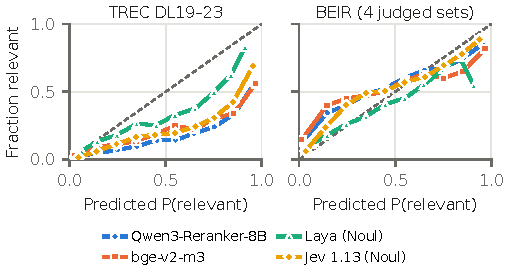
\includegraphics[width=\columnwidth]{figures/reliability.pdf}
\caption{Raw reliability on judged candidate pairs for bge, Qwen3-Reranker-8B, and the Noul readouts of Laya and Jev. Pooled within DL19--23 (left) and the four BEIR collections with negatives (right); 10 equal-width bins for readability (the ECE values in Table~\ref{tab:calibration} use 15 bins), hiding bins with fewer than 15 pairs. Noul needs no strict/lenient policy choice. Decision models are closer to the diagonal on DL; BEIR behavior is mixed.}
\label{fig:reliability}
\end{figure}

\subsection{RQ2: Calibration}

Raw cross-encoder scores were never trained to be probabilities, so a raw comparison mainly asks whether a model can be thresholded \emph{out of the box}. The fairer comparison is with \emph{transfer} calibration, which fits Platt scaling on other collections and uses no labels of the target collection (Table~\ref{tab:calibration}). We lead with the Noul readout, which needs no strict/lenient choice, and with the strict readout applied everywhere; the per-collection readout policy, chosen after observing TREC-COVID (\emph{Probability readout}), is reported as a sensitivity analysis.

\emph{Out of the box, Jev and Laya yes/no probabilities are better calibrated than raw cross-encoder scores.}
Jev Noul has mean ECE 5.0 points below bge (paired query-bootstrap 95\% CI $[-6.3,-3.9]$), lower on eight of nine collections, significantly lower on five after Holm, and significantly higher on none (TREC-COVID is slightly higher, $+0.17$). Laya Noul is 9.2 points lower ($[-10.8,-7.5]$). Jeff Noul is the exception (25.6 versus bge 20.0). On DL, the trained rerankers over-predict relevance (ECE 51.1/36.5/27.6 for Qwen0.6B/4B/8B, 47.0 for MiniLM, and 23.1 for bge; Figure~\ref{fig:reliability}).
The advantage depends on the readout for the graded formats. With the strict readout everywhere, Jev C3 is only 0.7 points below bge ($[-2.5,0.9]$) and Jev S4 2.1 points below ($[-3.4,-0.9]$); under the per-collection policy, Jev C3 is 5.1 points below ($[-7.1,-3.4]$), while Jev S4 over-predicts relevance (mean prediction 0.55 against a base rate of 0.31) because the lenient readout $P(\ell\ge1)$ counts ``related but not answering'' as relevant. Jev's DBPedia ECE is worse than bge's by 9.9 under the policy and 14.1 under strict, and Robust04 by 0.9 under both.
These differences change by at most 0.4 points with 5--30 bins or equal-mass binning. A Brier decomposition attributes Jev Noul's advantage to both reliability (0.043 vs.\ 0.067) and resolution (0.066 vs.\ 0.045).

\emph{Transfer calibration closes the gap.}
Pooling all other collections (pair-weighted) yields ECE 14.9 for bge and 16.8 for MiniLM, versus Jev C3/S4/Noul 15.1/14.8/14.2 and Laya C3 11.0 under the strict readout (9.1/8.2 for Jev C3/S4 and 7.5 for Laya C3 under the per-collection policy); collection-balanced pooling changes little. Restricting sources to collections with the same numeric relevance threshold (DL$\to$DL and BEIR$\to$BEIR, collections weighted equally) yields bge 6.9, essentially equal to Jev Noul at 6.8, slightly below Jev S4 (7.5), and below Jev C3 (9.1) and Laya C3 (9.6). The BEIR group mixes partial-relevance definitions with strict Robust04, so it approximates rather than matches target relevance semantics.
The practical advantage of decision-model probabilities is therefore that they need no labelled source collections, not that they are better calibrated than a cross-encoder with a cheap transfer fit.

\emph{Raw calibration depends on the prompt wording.} Rewording the question while keeping its meaning moves raw ECE far more than ranking (Supplementary Material, \emph{Prompt sensitivity}): for Jev Noul, three paraphrases give 7.5--25.9 on DL19 (original 12.4) and 14.3--34.5 on DL20 (20.7), while nDCG@10 stays within 2.7 points; Qwen3-Reranker-0.6B's default instruction is its least calibrated wording, and Qwen3-235B's original prompt its best calibrated. The 5-point raw-ECE gap between Jev Noul and bge is thus smaller than the spread that rewording alone produces, and its direction could change under another prompt. We report it as a property of the prompts we used, not of decision models in general.

\emph{Other models.} On the seven collections where Clef was run, Clef C3 has raw ECE 12.3 and Brier 0.167 under the strict readout, versus Jev C3 16.6 and bge 20.2; the per-collection policy, which differs only on TREC-COVID for these collections, lowers Clef C3 to 7.8 and Jev C3 to 12.5. On the same seven collections, Clef Noul has ECE 12.5 versus 12.1 for its base. Jeff Noul has ECE 25.6 versus 26.5 for its base across nine collections, and Jeff C3 13.9 (15.3 under the policy). Qwen235B's raw yes/no ECE is 20.5, which transfer reduces to 10.5, versus Jev Noul 13.0 on the same collections.

\emph{Pool dependence.} Calibration is measured on judged candidates, whose mean base rate is 0.31. Treating unjudged candidates as non-relevant preserves the raw advantage of Jev Noul and Laya Noul but reverses that of Jeff C3 under either readout (Supplementary Table~S3).

\subsection{Efficiency}

Per query--passage pair, the local cross-encoders and Qwen3-Reranker-0.6B take 0.3--14\,ms (median) on a laptop GPU, Qwen3-Reranker-4B and 8B 102 and 148\,ms (4-bit), Laya 58\,ms, and Jeff 100\,ms (with slow reference kernels); the API models take a median 176\,ms (Jev), 401\,ms (Clef), and 850\,ms (Qwen3-235B) per call with 8--24 concurrent requests. Reranking 100 passages costs \$3.4 per 1k queries with Jev on average (\$2.4--5.7; long documents cost more) and \$2.3 with the Qwen3-235B yes/no baseline; on the seven collections where both were run, Clef 27B costs about 4.8 times as much as Jev (\$15.3 vs.\ \$3.2). Local and API latencies come from different hardware, serving stacks, and concurrency levels, so they indicate orders of magnitude rather than a controlled speed comparison.

\begin{table*}[t]
\centering
\footnotesize
\setlength{\tabcolsep}{4pt}
\caption{RQ3 on the family-disjoint MuSiQue split: answer F1 on the 597 final questions (88\% 2-hop) whose decomposition families share no sub-question with the calibration split or the original pilot. Policies and thresholds are those locked after the original pilot; Platt scaling and Jev's readout are refit on the family-disjoint calibration split. $^\dagger$: Jev significantly better than bge-reranker-v2-m3 under the same policy (question-level paired $t$-test, Holm-corrected, $p<0.05$). Family-bootstrap intervals are given in the text. $^\ddagger$: Jev significantly better than Qwen3-Reranker-8B under the same policy (same test and correction, added after final results).}
\label{tab:rag-fd}
\begin{tabular}{lrrrr}
\toprule
 & \multicolumn{3}{c}{MuSiQue} & Avg.\ $n$ \\
Policy & Qwen2.5-7B & Llama-3.1 & Qwen3-30B &  \\
\midrule
No context & 13.5 & 10.4 & 20.2 & 0.0 \\
All 20 passages & 40.8 & 38.5 & 51.1 & 20.0 \\
Gold passages (oracle) & 62.0 & 58.7 & 68.6 & 2.1 \\
\multicolumn{5}{l}{\textit{Jev 1.13}} \\
\quad top-1 & 39.7$^\dagger$$^\ddagger$ & 33.0$^\dagger$$^\ddagger$ & 42.1$^\dagger$$^\ddagger$ & 1.0 \\
\quad top-3 & 45.5$^\dagger$$^\ddagger$ & 42.3$^\dagger$ & 51.8$^\dagger$$^\ddagger$ & 3.0 \\
\quad top-5 & 44.2$^\dagger$ & 40.4$^\dagger$ & 51.7 & 5.0 \\
\quad adaptive-$k$ & 42.6$^\dagger$$^\ddagger$ & 39.1$^\dagger$$^\ddagger$ & 48.9$^\dagger$$^\ddagger$ & 2.3 \\
\quad $P>0.3$ & 38.2$^\dagger$ & 35.6$^\dagger$ & 44.0$^\dagger$ & 1.7 \\
\quad top-2 $+$ $P>0.3$ & 44.0$^\dagger$$^\ddagger$ & 40.5$^\dagger$ & 49.8$^\dagger$ & 2.5 \\
\multicolumn{5}{l}{\textit{bge-reranker-v2-m3}} \\
\quad top-1 & 22.8 & 20.9 & 28.8 & 1.0 \\
\quad top-3 & 40.3 & 34.4 & 46.0 & 3.0 \\
\quad adaptive-$k$ & 30.0 & 27.3 & 36.2 & 3.0 \\
\quad top-2 $+$ $P>0.3$ & 36.3 & 31.8 & 43.2 & 2.8 \\
\multicolumn{5}{l}{\textit{Qwen3-Reranker-8B (4-bit)}} \\
\quad top-1 & 30.0 & 26.7 & 35.7 & 1.0 \\
\quad top-3 & 39.8 & 38.0 & 46.8 & 3.0 \\
\quad adaptive-$k$ & 35.2 & 34.0 & 41.9 & 3.4 \\
\quad top-2 $+$ $P>0.3$ & 39.4 & 37.0 & 47.2 & 3.0 \\
\multicolumn{5}{l}{\textit{Qwen3-Reranker-0.6B}} \\
\quad top-1 & 23.8 & 20.9 & 27.8 & 1.0 \\
\quad top-3 & 35.0 & 32.7 & 41.6 & 3.0 \\
\quad adaptive-$k$ & 31.6 & 27.8 & 36.8 & 3.2 \\
\quad top-2 $+$ $P>0.3$ & 33.5 & 29.8 & 37.6 & 2.7 \\
\bottomrule
\end{tabular}
\end{table*}

\begin{table*}[t]
\centering
\footnotesize
\setlength{\tabcolsep}{4pt}
\caption{RQ3: answer F1 on the original 1{,}000 ID-disjoint final questions per dataset; MuSiQue component families overlap design splits. Avg.\ $n$: mean number of selected passages (independent of generator). $^\dagger$: Jev significantly better than bge-reranker-v2-m3 under the same policy in the original question-level paired $t$-test (Holm-corrected, $p<0.05$); these tests do not account for family dependence. $^\ddagger$: Jev significantly better than Qwen3-Reranker-8B under the same policy (same test and correction, added after final results). Displayed policies and ranker-effect comparisons were fixed after separate pilot questions. Thresholds use a readout selected with labelled calibration questions; the $P>0.3$ rows are Platt-scaled.}
\label{tab:rag}
\begin{tabular}{lrrrrrrrr}
\toprule
 & \multicolumn{3}{c}{MuSiQue} & \multicolumn{3}{c}{NQ} & \multicolumn{2}{c}{Avg.\ $n$} \\
Policy & Qwen2.5-7B & Llama-3.1 & Qwen3-30B & Qwen2.5-7B & Llama-3.1 & Qwen3-30B & MuSiQue & NQ \\
\midrule
No context & 10.5 & 9.3 & 12.6 & 26.7 & 31.4 & 35.2 & 0.0 & 0.0 \\
All 20 passages & 38.8 & 37.0 & 46.3 & 52.5 & 49.4 & 51.5 & 20.0 & 20.0 \\
Gold passages (oracle) & 60.9 & 54.7 & 64.1 & 60.2 & 59.1 & 59.7 & 2.6 & 3.4 \\
\multicolumn{9}{l}{\textit{Jev 1.13}} \\
\quad top-1 & 45.2$^\dagger$$^\ddagger$ & 36.4$^\dagger$$^\ddagger$ & 43.4$^\dagger$$^\ddagger$ & 50.4$^\ddagger$ & 50.4$^\dagger$$^\ddagger$ & 51.4$^\ddagger$ & 1.0 & 1.0 \\
\quad top-3 & 44.6$^\dagger$$^\ddagger$ & 39.3$^\dagger$$^\ddagger$ & 47.1$^\dagger$$^\ddagger$ & 52.1 & 50.5 & 52.9 & 3.0 & 3.0 \\
\quad top-5 & 42.4$^\dagger$ & 40.7$^\dagger$$^\ddagger$ & 47.9$^\dagger$$^\ddagger$ & 51.9 & 50.9 & 53.0 & 5.0 & 5.0 \\
\quad adaptive-$k$ & 46.7$^\dagger$$^\ddagger$ & 40.2$^\dagger$$^\ddagger$ & 47.2$^\dagger$$^\ddagger$ & 52.3 & 50.1 & 52.3 & 2.9 & 6.2 \\
\quad $P>0.3$ & 43.6$^\dagger$$^\ddagger$ & 36.1$^\dagger$$^\ddagger$ & 43.5$^\dagger$$^\ddagger$ & 51.2 & 51.5 & 52.3 & 2.4 & 2.9 \\
\quad top-2 $+$ $P>0.3$ & 44.2$^\dagger$$^\ddagger$ & 39.1$^\dagger$$^\ddagger$ & 45.2$^\dagger$$^\ddagger$ & 51.8 & 51.0 & 53.2 & 3.0 & 3.5 \\
\multicolumn{9}{l}{\textit{bge-reranker-v2-m3}} \\
\quad top-1 & 22.0 & 18.0 & 23.7 & 47.9 & 47.1 & 49.1 & 1.0 & 1.0 \\
\quad top-3 & 38.5 & 31.5 & 39.1 & 51.4 & 50.5 & 52.6 & 3.0 & 3.0 \\
\quad adaptive-$k$ & 30.5 & 26.1 & 32.6 & 50.6 & 50.5 & 51.8 & 3.1 & 7.1 \\
\quad top-2 $+$ $P>0.3$ & 35.7 & 30.4 & 37.9 & 51.3 & 51.2 & 52.6 & 2.9 & 3.9 \\
\multicolumn{9}{l}{\textit{Qwen3-Reranker-8B (4-bit)}} \\
\quad top-1 & 30.6 & 25.2 & 31.6 & 47.4 & 45.6 & 47.8 & 1.0 & 1.0 \\
\quad top-3 & 40.3 & 34.0 & 44.3 & 50.9 & 50.4 & 52.2 & 3.0 & 3.0 \\
\quad adaptive-$k$ & 37.6 & 32.8 & 38.6 & 51.2 & 50.3 & 51.7 & 3.7 & 10.3 \\
\quad top-2 $+$ $P>0.3$ & 38.7 & 35.2 & 41.1 & 51.3 & 50.4 & 51.3 & 3.1 & 4.4 \\
\multicolumn{9}{l}{\textit{Qwen3-Reranker-0.6B}} \\
\quad top-1 & 23.8 & 19.2 & 23.5 & 42.2 & 42.2 & 44.2 & 1.0 & 1.0 \\
\quad top-3 & 34.6 & 29.7 & 36.2 & 49.1 & 47.6 & 49.9 & 3.0 & 3.0 \\
\quad adaptive-$k$ & 30.9 & 27.6 & 33.1 & 50.9 & 49.4 & 50.6 & 3.2 & 10.1 \\
\quad top-2 $+$ $P>0.3$ & 31.9 & 29.2 & 34.8 & 49.9 & 47.8 & 50.7 & 2.8 & 3.8 \\
\bottomrule
\end{tabular}
\end{table*}

\subsection{RQ3: Context selection}

Table~\ref{tab:rag-fd} reports answer F1 on the 597 family-disjoint MuSiQue final questions, our primary multi-hop result; Table~\ref{tab:rag} reports the original 1{,}000-question final splits of MuSiQue and NQ.

\emph{Better ranking improves multi-hop answers.} On the family-disjoint MuSiQue split, passages selected by Jev beat those selected by bge-reranker-v2-m3 under every policy and with every generator, by $+2.8$ to $+16.9$ F1. Twenty-three of the 27 comparisons (nine policies, three generators) pass the family-clustered Holm test (Supplementary Table~S9; 26 pass question-level Holm, and 26 have family-bootstrap 95\% intervals excluding zero). The four that do not are top-3 and top-5 with Qwen2.5-7B (Holm $p=0.06$) and top-5 and $P>0.2$ with Qwen3-30B; only top-5 with Qwen3-30B ($+2.8$, $[-0.6,6.1]$) has a family-bootstrap interval that includes zero. Exact match agrees in direction: Jev's EM exceeds bge's in all 27 comparisons, 18 of them significant with family clustering. The gains are largest when few passages are selected: top-1 $+12.1$ to $+16.9$ and Adaptive-$k$ $+11.8$ to $+12.7$, against $+5.2$ to $+7.8$ for top-3 and $+2.8$ to $+3.6$ for top-5. With every generator, Jev's top-3 (45.5, 42.3, 51.8) is at least as good as giving the generator all 20 candidates (40.8, 38.5, 51.1) with a fifth of the generator input tokens (491 vs.\ 2{,}676 for Qwen2.5-7B, excluding the cost of scoring the candidates). On NQ, despite Jev's higher recall of answer-bearing passages (R@3 58.4 vs.\ 52.5; Supplementary Table~S4), only one of 27 comparisons is significant.

\emph{Sensitivity: the original split.} On the original MuSiQue split, whose final questions share decomposition sub-questions with the calibration or pilot splits (Experimental Setup, \emph{RQ3: context selection}), Jev's gains are somewhat larger ($+2.6$ to $+23.2$ F1; top-1 $+18.5$ to $+23.2$) and all 27 comparisons pass question-level Holm (26 with family clustering; this split contains 365 families). Exact match shows the same pattern there (Supplementary Table~S5): Jev's EM exceeds bge's in all 27 policy--generator pairs, by 2.6 to 21.7 points, and 26 pass Holm with either test; on NQ, none does. On the retrospective subset of 329 original final questions that share no sub-question ID with either design split (Supplementary Table~S6), the top-1 and Adaptive-$k$ gains ($+10.7$ to $+18.8$) hold for every generator with family intervals excluding zero, while the top-3 gains shrink to $+2.4$ to $+5.7$. The family-disjoint split differs from the original one in hop mix as well as overlap (88\% vs.\ 52\% 2-hop), so the smaller effects do not measure overlap-induced inflation alone; they do show that the ranking advantage does not depend on shared sub-questions. Nor is the gain specific to 2-hop questions: on the original split, Jev's advantage over bge is on average larger on 3- and 4-hop questions (mean over the 27 policy--generator pairs $+8.3$, $+11.2$, and $+15.3$ F1 for 2, 3, and 4 hops; top-1 $+18.8$ to $+28.8$ F1 versus $+16.8$ to $+19.8$ on 2-hop; Adaptive-$k$ $+13.7$ to $+27.5$ versus $+11.3$ to $+12.8$), and unadjusted question-level 95\% intervals exclude zero in 77 of the 81 hop--policy--generator cells (\texttt{results/rag\_hop\_f1.csv}). On the family-disjoint split the gain over bge is likewise larger on its 58 three-hop questions (16 families; mean over the 27 pairs $+20.6$ F1, family-clustered 95\% intervals excluding zero in 21) than on its 526 two-hop questions ($+6.9$; 23 of 27), whereas its 13 four-hop questions come from three families and support no estimate.

\emph{The gain is not only that of a stronger reranker.} On the original split (Table~\ref{tab:rag}), Qwen3-Reranker-8B, which ranks about as well as Jev in RQ1, recovers part of Jev's MuSiQue advantage over bge (top-1: 30.6, 25.2, and 31.6 F1 versus bge's 22.0, 18.0, and 23.7), but Jev beats it under every policy with every generator ($+1.6$ to $+14.5$ F1; top-1 $+11.3$ to $+14.5$, Adaptive-$k$ $+7.4$ to $+9.1$), and 26 of 27 comparisons pass question-level Holm (the exception is top-5 with Qwen2.5-7B, $+1.6$, $p=0.18$), but only 19 pass the family-clustered test; the eight that do not are mostly top-5 and threshold policies. On NQ, Jev beats Qwen8B only at top-1 ($+3.1$ to $+4.8$ with every generator); the other 24 differences lie between $-0.1$ and $+2.6$ and are not significant after Holm. Qwen3-Reranker-0.6B is below Jev in all 27 comparisons on both MuSiQue and NQ (significant after Holm in 27 and 18). These comparisons were added after the final results; they are marked $^\ddagger$ in Table~\ref{tab:rag}. On the family-disjoint split (Table~\ref{tab:rag-fd}) the margin over Qwen8B is smaller but keeps its direction. Qwen8B again recovers part of the gap to bge (top-1: 30.0, 26.7, and 35.7 F1 versus bge's 22.8, 20.9, and 28.8), and Jev is ahead in 26 of 27 comparisons ($-0.2$ to $+9.7$ F1; top-1 $+6.4$ to $+9.7$, Adaptive-$k$ $+5.1$ to $+7.4$). Twelve pass the family-clustered Holm test (14 question-level), 16 have family-bootstrap intervals excluding zero, and none favors Qwen8B; most of the others are top-5 or pure-threshold policies. In exact match Jev is ahead of Qwen8B in 25 of 27 comparisons, five of them significant. Qwen3-Reranker-0.6B is below Jev in all 27 ($+5.1$ to $+15.9$).

\emph{Jev ranks the answer-bearing hop first.} On the original split, the ranking advantage coincides with a difference in \emph{which} passage each ranker puts first. bge-reranker-v2-m3's top passage is a supporting paragraph slightly more often (88.0\% vs.\ 82.2\%, McNemar $p<10^{-4}$), but usually the first hop---the one that shares the question's entities (61.9\%)---whereas Jev's top passage is the last, answer-bearing hop in 51.2\% of questions against 15.2\% ($p<10^{-80}$; Supplementary Table~S4), and 51--60\% across Jev's three readouts. The pattern replicates on the family-disjoint split: Jev S4's top passage is the last hop in 46.1\% of questions versus 15.9\% for bge and 29.0\% for Qwen8B (family-clustered differences $+30.2$, 95\% CI $[24.3,36.0]$, and $+17.1$, $[11.6,22.6]$) and contains the answer in 50.6\% versus 22.1\% and 34.8\%, while bge and Qwen8B put some supporting paragraph first slightly more often (87.4\% and 88.3\% vs.\ 82.9\%).
This preference is not reproduced by rewording a label-probability reranker's instruction: asking Qwen0.6B whether the passage is relevant, answers, or contains the answer yields only 16.5--18.4\% last-hop@1 and 51--56\% first-hop@1. Qwen3-Reranker-8B lies in between: its top passage is the last hop in 30.2\% of questions and the first hop in 44.5\%, and contains the answer in 36.6\% (Jev 56.5\%, bge 22.3\%). Its top-3 recall of supporting paragraphs equals Jev's (68.6\% vs.\ 68.7\%), yet Jev's top-3 contexts score 2.8--5.3 F1 higher, consistent with which supporting paragraph is selected mattering more than how many.
Replacing gold-answer strings with \texttt{[MASKED]} reduces Jev S4 last-hop@1 to 43.8\% (Noul: 50.3\%) from 51.2\% (56.4\%); masked bge scores 13.4\%. Because the marker itself reveals answer location (it appears in 999 of 1{,}000 last-hop paragraphs but only 1{,}621 of 19{,}988 candidates), this perturbation cannot separate question resolution from that cue, prior entity knowledge, or memorized chains.

\emph{Thresholds on probabilities do not beat fixed $k$.} A pure threshold at 0.3 on Platt-scaled probabilities leaves the generator with no passage for 10.3\% of MuSiQue and 21.6\% of NQ questions, which then fall back to closed-book answering (the prompt does not allow abstention). Raw $P>0.3$ is within 1.3 F1 of the Platt threshold and of top-3 on NQ for every generator; on MuSiQue it selects nothing for 25\% of questions and is 3.4--5.9 F1 below top-3 (Supplementary Material, \emph{Raw-probability thresholds}).
The top-2+threshold rule is within $\pm2$ F1 (TOST) of top-2, top-3, top-5, and Adaptive-$k$ on NQ for every generator. On MuSiQue it is equivalent to top-2 (and, for Llama, to top-3), but pooled over generators it is 1.9 F1 below Adaptive-$k$ (95\% CI $[-3.4,-0.4]$; Holm-adjusted $p=0.065$), and individual comparisons against Adaptive-$k$, top-3, and top-5 trend lower by 1.9--2.7 F1 (unadjusted $p=0.01$--$0.05$, none significant after Holm). On the family-disjoint split it is 1.5--2.0 F1 below top-3 and 0.9--1.4 F1 above Adaptive-$k$, with no comparison passing Holm and every family interval crossing zero; it is equivalent to top-2 for Llama and Qwen3-30B and pooled over generators (TOST $p<0.05$). A pure Platt threshold at 0.3 leaves 16.2\% of these questions without context. Because it selects more than two passages for 39\% of MuSiQue and 45\% of NQ questions (3.0 and 3.5 on average), it also saves no tokens over top-3.
These results do not show that better-calibrated probabilities fail to help, because on the RAG final sets Jev's probabilities are not the better calibrated ones (Supplementary Table~S10): after Platt scaling fit on the calibration split, ECE on the family-disjoint final pairs is 3.1 for Jev Noul (question-bootstrap 95\% CI $[2.8,3.7]$) versus 1.3 ($[0.9,1.9]$) for bge and 1.4 for Qwen8B, and on NQ 3.8 for Jev Choice-3 versus 1.4 for bge (Jev Noul, not selected by the Brier criterion, reaches 1.2). Jev also ranks by Score-4 but thresholds another readout, so its passages with $P>0.3$ are not a prefix of its ranking for 10.7\% of family-disjoint MuSiQue questions (21.8\% on the original split, 5.0\% on NQ). Compared with fixed top-$k$ interpolated to the same average number of passages, $P>0.3$ is 2.4--4.0 F1 lower on the family-disjoint split for every generator, while top-2+threshold is within 0.8 F1.
Jev's practical advantage for RAG is therefore its ranking, not thresholding on its probabilities.

\section{Threats to Validity}

\subsection{Pre-specified versus post-hoc analyses}

Several analyses were added or changed after results were observed, and we flag them here in one place. (i)~The per-collection strict/lenient readout policy was introduced after observing a Choice-3 ECE of 43.9 on TREC-COVID; we therefore lead with the policy-free Noul readout and the strict-everywhere readout, and give both readouts for every collection (Supplementary Table~S2). (ii)~The $\pm2$ nDCG and $\pm2$ F1 equivalence margins, the TOST analyses, and the modified Knapp--Hartung sensitivity analysis are post-hoc and exploratory. (iii)~In RQ3, threshold-rule comparisons against top-3 and Adaptive-$k$ were fixed after the pilot; comparisons against top-2 and top-5 and the raw (non-Platt) thresholds were added after final results. (iv)~The 329-question MuSiQue subset is a retrospective sensitivity analysis on existing outputs, not a new confirmatory split. (v)~Added during revision, after the original results were known: the family-disjoint MuSiQue split, the downstream comparison with Qwen3-Reranker-8B/0.6B, the strict readout as the primary calibration row for every Choice-3 and Score-4 system, the extension of the Clef base control from three to seven collections, the 4{,}000-character Qwen3-Reranker-8B control, the prompt paraphrases, the SPLADE++ first stage and its pool-coverage check, the per-hop F1 breakdown, and the exact-match tables. The policies, thresholds, and paraphrases were fixed before the corresponding runs, but the decision to run each analysis was not. (vi)~Added in response to peer review, from existing outputs or local models: family-clustered tests as the primary MuSiQue inference, the completion range of the DL19 SPLADE++ difference, prediction intervals, the held-out calibration of the RAG probabilities, the rank/threshold mismatch and equal-size top-$k$ comparison, the judged-count table, the family-disjoint mechanism, exact-match, and hop analyses, the threshold comparison for every ranker, and the 4{,}000-character Qwen3-Reranker-8B runs on TREC-COVID, NFCorpus, and SciFact.

\subsection{Statistical dependence}

The three question formats of each decision model are answered in one call per pair and are not independent samples. Holm correction is applied within each system--baseline pair across collections, not across the 22 systems and formats (75 system--baseline pairs). The original MuSiQue split was by ID, and 671 of 1{,}000 final questions share at least one decomposition sub-question with the calibration or pilot splits. Our primary family-disjoint split removes this overlap, and our primary MuSiQue tests cluster questions by family, but the split was built after the original results were seen, and excluding every family that reaches the pilot leaves a split that is 88\% 2-hop, so its results speak mainly to 2-hop questions.

\subsection{Configurations rather than isolated effects}

Same-base comparisons differ in prompts and context budgets (4{,}000 characters for Jev, Clef, and Jeff; 448 tokens for the label-probability controls), so they compare configurations rather than isolate decision-model training. Qwen3-Reranker-4B/8B use 4-bit weights. Clef and Qwen3-235B cover subsets of collections, and the Clef base control covers Clef's seven. The main results use a single prompt per format; across four wordings of the question, raw DL calibration error spans up to 17 points for Qwen3-Reranker-0.6B, 13 for Qwen3-235B, and 20 for Jev Noul, while nDCG@10 spans at most 2.7 (Supplementary Material, \emph{Prompt sensitivity}). Latencies come from different hardware and serving stacks.

\subsection{Benchmarks and contamination}

Our main experiments use BM25 candidates; on SPLADE++ candidates Jev's DL19 deficit to the cross-encoders cannot be separated from incomplete judgments, so first-stage effects are confounded with pool coverage (Supplementary Material, \emph{Neural first stage}). Calibration is measured on judged candidates, and numeric-threshold transfer groups need not share identical relevance semantics. We retain the DL23 synthetic queries and DL22 propagated judgments. Jev is a closed model whose size, training data, and cutoff are unknown; Robust04, MuSiQue, NovelEval, and FutureQueryEval all predate its release, so contamination cannot be excluded, and the answer-masking perturbation cannot separate reasoning from memorization. The RAG comparison covers bge-reranker-v2-m3 and Qwen3-Reranker-8B/0.6B but not the API label-probability baselines, the Qwen comparisons were added after the final results, thresholds use target calibration labels, and the generator cannot abstain.

\section{Conclusion}

Large typed decision models are competitive pointwise passage rerankers: Jev is on par with Qwen3-Reranker-8B and ahead of bge-reranker-v2-m3 on average, with large variation across collections (on SPLADE++ candidates it trails on DL19 under standard scoring, a deficit that cannot be separated from incomplete judgments), and its gains over bge persist at equal passage budgets on News and Robust04, as does its Robust04 lead over Qwen3-Reranker-8B when both read the same 4{,}000 characters (Qwen3-Reranker-8B stays ahead on Touche and News). Same-base controls suggest that Clef's effectiveness comes largely from its underlying LLM: it does not differ significantly from its base on six of seven collections and is ahead only on Robust04, where the base reads less text, while the small Jeff model improves on its base; Jev's base model is unknown, so we cannot attribute its effectiveness either way.
Out of the box, the yes/no probabilities of Jev and Laya are better calibrated than raw cross-encoder scores (Jeff's are not better than bge's, and Jev's graded formats depend on the readout), but a cross-encoder calibrated on other collections with the same relevance threshold reaches similar error; their practical advantage is that no labelled source data are needed, and rewording the prompt moves raw calibration error by more than the gap to bge. Small open decision models remain weak deep rerankers under standard evaluation.
For RAG, Jev improves multi-hop answer quality over bge with all three generators, and also over Qwen3-Reranker-8B despite equal ranking effectiveness, and it more often ranks the answer-bearing final hop first; on a family-disjoint MuSiQue split the gains remain ($+2.8$ to $+16.9$ F1 over bge, 23 of 27 comparisons significant with family-clustered tests; over Qwen8B, 12 of 27), largest when few passages are selected. Thresholding its probabilities, however, does not improve over fixed top-$k$ selection. Calibration alone, in short, does not make context selection a simple threshold.
Future work should build family-disjoint multi-hop splits with more 3- and 4-hop questions, extend the downstream comparison to the API label-probability baselines, and match context budgets across models on all collections.

% Acknowledgements and Statements and Declarations are on the separate title page (double-anonymized review)

% SAGE Vancouver, the reference style of the Journal of Information Science
\bibliographystyle{SageV}
\bibliography{refs}

% The appendix is uploaded separately as supplementary material (supplementary.tex).
\end{document}
